\documentclass[xcolor=svgnames]{beamer}
\mode<presentation>
{
      \setbeamertemplate{footline}[page number]
      \setbeamercovered{transparent}
      \setbeamertemplate{navigation symbols}{}
      \usecolortheme[named=DarkGreen]{structure}
}

\usepackage[english]{babel}
\usepackage{times}
\usepackage{url}
\usepackage{CJKutf8}
\usepackage{graphics}

\begin{document}
\begin{CJK*}{UTF8}{gbsn}


\title{操作系统概论}


\begin{frame}{操作系统的作用}
\begin{itemize}
\item 提供容易使用的界面(终端用户及程序员)
\item 最大限度地提高资源利用率(CPU,内存)
\item 为多用户提供分时服务(time sharing system)
\item 在多用户多系统之间实现资源共享(存储、打印机)
\item 嵌入式设备:界面问题、电池寿命问题(不只是OS的任务)
\end{itemize}
\end{frame}

\begin{frame}{操作系统的作用: 提供易于使用的界面}
%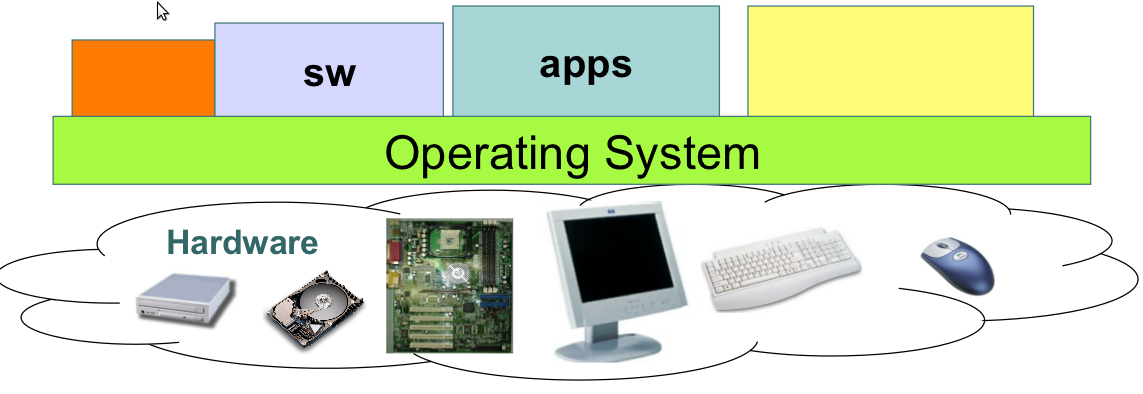
\includegraphics[width=1.0\textwidth]{os-function.png}
\begin{columns}
\column{.5\textwidth}
磁盘读写操作:
\begin{itemize}
\item 磁头、柱面、磁道、扇区
\item 读写前需等待机械运动结束
\item 数据存储可能不连续
\item 磁盘大小、速度各不相同
\item 对程序员而言, 编程读写磁盘数据是非常复杂的任务
\end{itemize}

操作系统提供的磁盘读写界面:
\begin{itemize}
\item open(), close()
\item read(), write()
\item named files(按名访问)
\end{itemize}

\column{.5\textwidth}
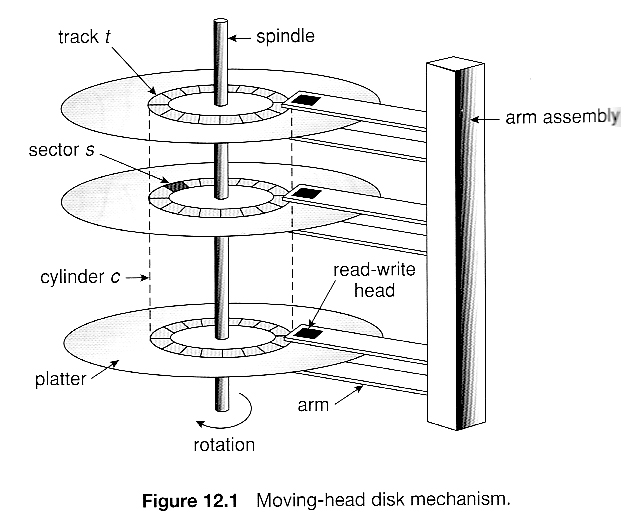
\includegraphics[width=1.0\textwidth]{disk.jpg}
\end{columns}
\end{frame}

\begin{frame}{操作系统的中断(interrupt)处理机制}
\begin{itemize}
\item 操作系统由中断驱动
\item 硬件中断与软件中断
\end{itemize}
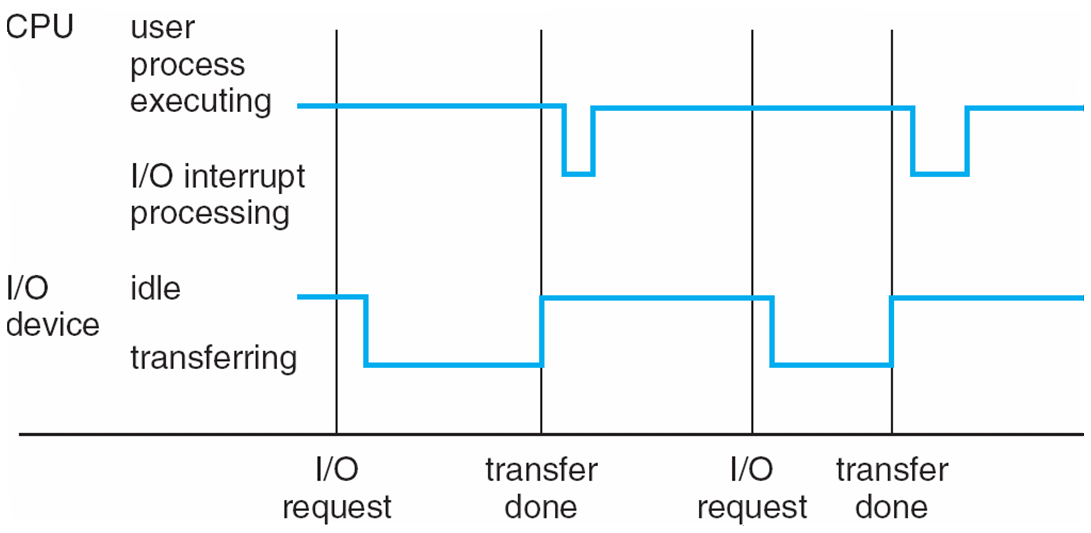
\includegraphics[width=1.0\textwidth]{interrupt.png}
\end{frame}

\begin{frame}{多道程序设计的概念}
\begin{columns}
\column{.3\textwidth}
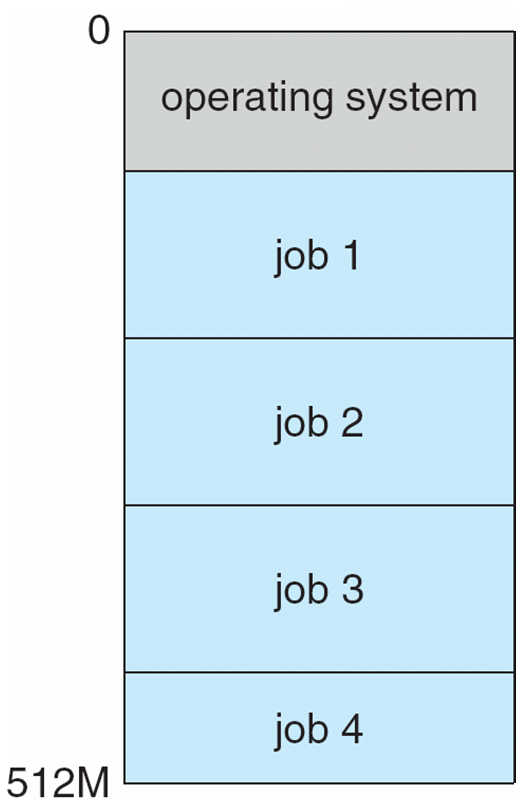
\includegraphics[width=1.0\textwidth]{jobs.png}
\column{.7\textwidth}
\begin{itemize}
\item 单个用户或程序无法使CPU或外设保持忙碌 
\item 引入多道程序设计技术
\item 多个作业(jobs)驻留内存
\item 操作系统需要进行作业调度
\item 需要等待I/O时,调入另一作业运行
\end{itemize}
\end{columns}
\end{frame}

\begin{frame}{核心态与用户态}
\begin{itemize}
\item 核心态: 执行操作系统代码
\item 用户态: 执行用户程序代码
\item 思考:哪些指令需要在核心态下执行?
\item 系统调用导致从用户态转入核心态
\end{itemize}
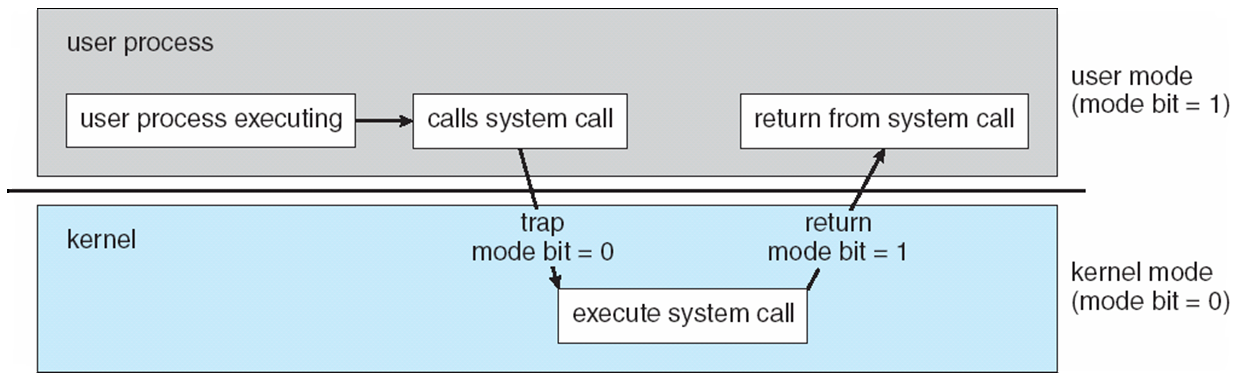
\includegraphics[width=1.0\textwidth]{mode.png}
\end{frame}

\begin{frame}{系统调用}
\begin{columns}
\column{.3\textwidth}
\begin{itemize}
\item CLI/GUI是人使用操作系统时的界面
\item 系统调用可看作获取操作系统服务的编程界面(接口)
\end{itemize}
\column{.7\textwidth}
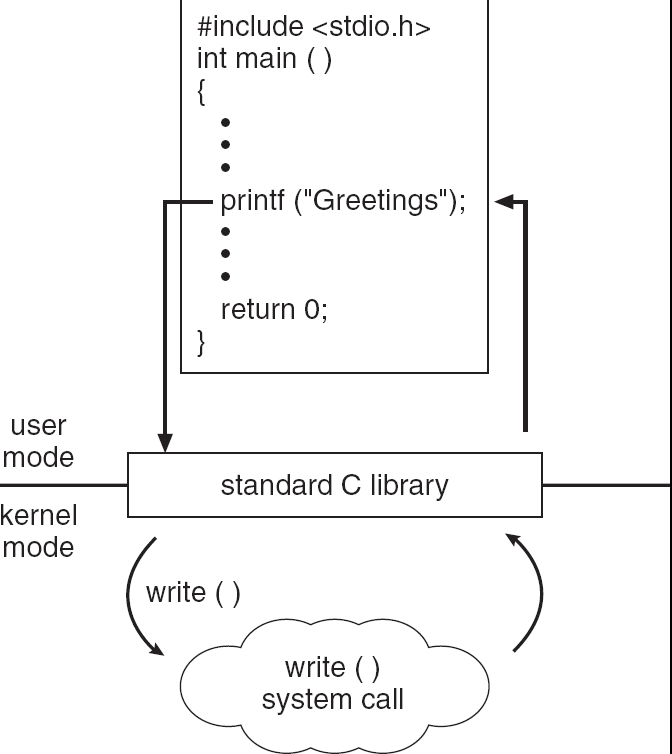
\includegraphics[width=0.8\textwidth]{printf.png}
\end{columns}
\end{frame}

\begin{frame}{进程概念}
\begin{columns}
\column{.5\textwidth}
\begin{itemize}
\item 操作系统执行用户程序
\begin{itemize}
\item 批处理系统 --- 作业
\item 分时系统 --- 用户程序、任务
\end{itemize}
\item 进程: 运行中的程序 
\item 进程包含三部分内容:
\begin{itemize}
\item 程序代码
\item 当前状态: 程序计数器以及寄存器
\item 栈(函数参数, 返回地址, 局部变量)
\item 数据区(全局变量)
\item 堆(动态分配的内存)
\end{itemize}
\end{itemize}
\column{.5\textwidth}
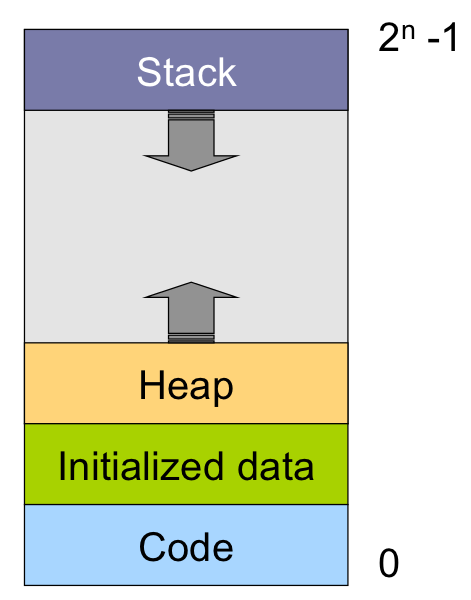
\includegraphics[width=1.0\textwidth]{memory.png}
\end{columns}
\end{frame}

\begin{frame}{进程的状态及其转移}
\begin{columns}%[t]
\column{.3\textwidth}
\begin{itemize}
\item new: 进程正在被创建
\item running: 正在运行
\item waiting: 挂起
\item ready: 就绪
\item terminated: 进程正在被销毁
\end{itemize}
\column{.7\textwidth}
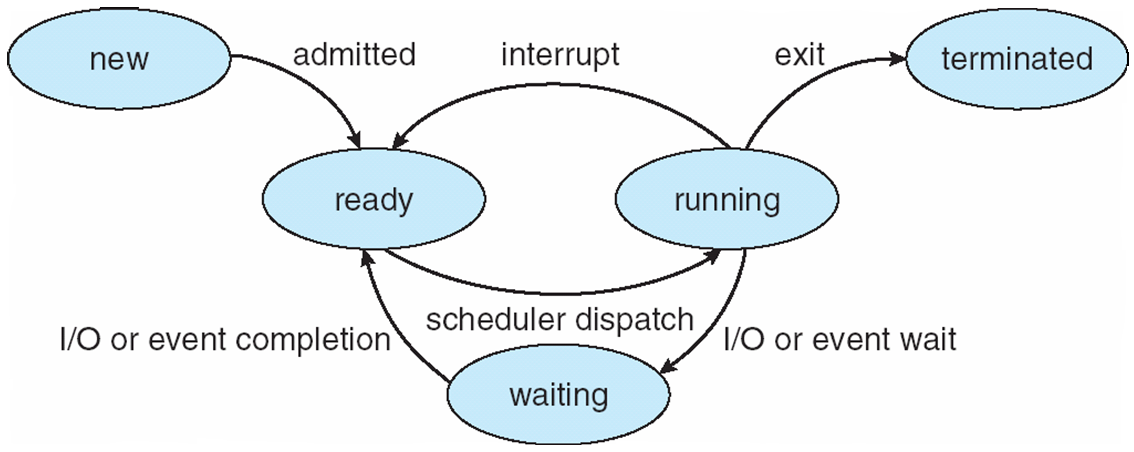
\includegraphics[width=1.0\textwidth]{state.png}
\end{columns}
\end{frame}

\begin{frame}{进程控制块(PCB)}
\begin{columns}%[t]
\column{.5\textwidth}
用于存放与每个进程相关的信息
\begin{itemize}
\item 进程状态
\item 程序计数器PC
\item CPU寄存器
\item CPU调度信息
\item 内存管理信息
\item I/O状态信息
\item 记账信息
\end{itemize}
\column{.5\textwidth}
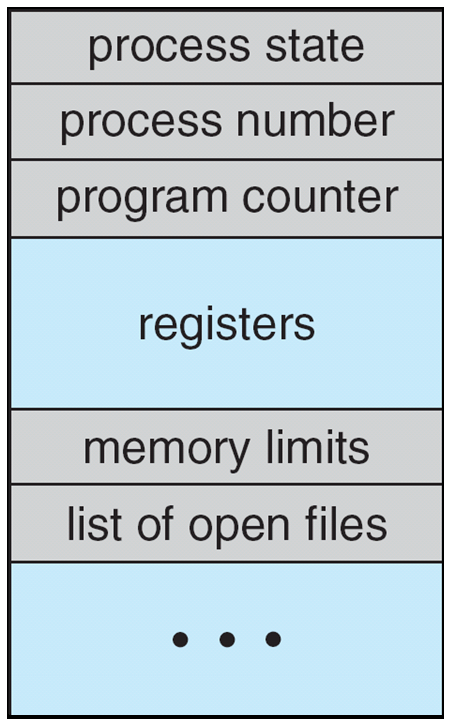
\includegraphics[width=0.6\textwidth]{PCB.png}
\end{columns}%[t]
\end{frame}

\begin{frame}{CPU在进程间切换}
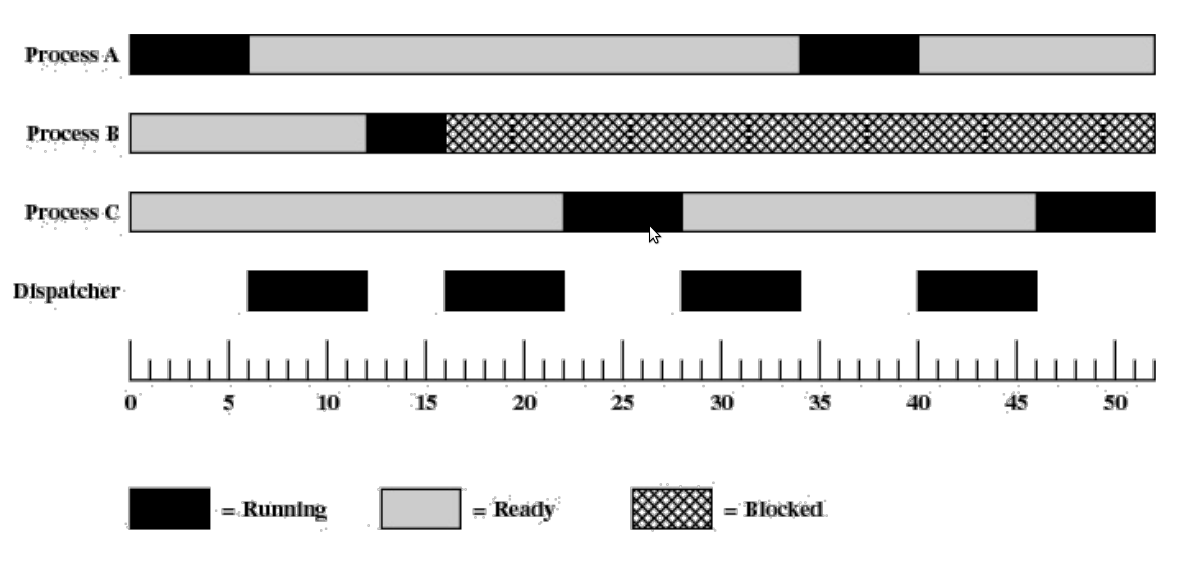
\includegraphics[width=1.0\textwidth]{dispatcher.png}
\end{frame}

\begin{frame}{上下文切换(context switch)}
\begin{itemize}
\item CPU分配给新进程时,原进程的状态需要保存,新进程的状态需要载入
\item 进程的上下文(context)保存于进程控制块(PCB)中
\item 上下文切换时间属无用开销,因此越快越好
\item 切换时间取决于硬件支持(e.g, 具有多组寄存器的CPU)
\end{itemize}
\end{frame}

\begin{frame}{线程的概念}
可以发现,进程概念可以分割成两块:
\begin{itemize}
\item 资源分配单位
\begin{itemize}
\item 内存空间
\item I/O设备,文件等
\end{itemize}
\item 执行单位
\begin{itemize}
\item 单一执行路径
\item 状态:寄存器、栈等
\end{itemize}
\item 重新定义术语的内涵:
\begin{itemize}
\item 进程:资源分配单位
\item 线程:执行单位(轻量级进程)
\item 多线程技术:支持一个进程中同时运行多个线程
\end{itemize}
\end{itemize}
\end{frame}

\begin{frame}{为什么引入多线程技术?}
\begin{itemize}
\item 应用程序可能同时执行多个动作(例如文字编辑器)
\item 线程比进程更容易创建和销毁
\item 如果程序部分因I/O阻塞,其余线程可以运行
\begin{itemize}
\item CPU密集型与I/O密集型并行
\item 加快系统速度
\end{itemize}
\item 充分利用多核处理器硬件资源
\end{itemize}
\end{frame}

\begin{frame}{临界资源、临界区与竞争条件}
\begin{itemize}
\item 临界资源
\item 临界区
\item 多个进程并发访问和操作同一数据且执行结果与访问的特定顺序有关,称为竞争条件。
\end{itemize}
\end{frame}

\begin{frame}{对临界资源的互斥访问}
理想的互斥方案需要满足4个条件:
\begin{enumerate}
\item[]
\item 两个进程不能同时进入临界区
\item[]
\item 不能依赖CPU数目或者运行速度
\item[]
\item 不在临界区的进程,不能妨碍其他进程进入临界区
\item[]
\item 任一进程需在有限时间内能够进入临界区
\end{enumerate}
\end{frame}

\begin{frame}{对临界资源的互斥访问: 忙等待}
\begin{columns}%[t]
\column{.5\textwidth}
\begin{itemize}
\item 需要硬件支持TSL指令
\item[]
\item 进程进入临界区前,调用enter\_region
\item[]
\item 离开临界区时,调用leave\_region
\item[]
\item 这是一个正确的解决方法,但是 ...
\end{itemize}
\column{.5\textwidth}
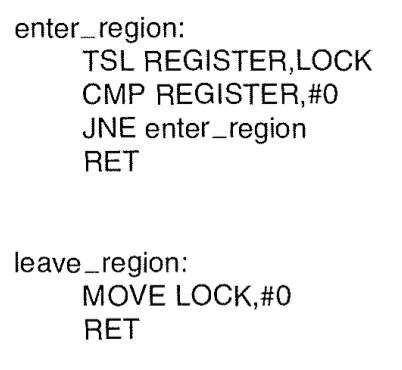
\includegraphics[width=1.0\textwidth]{tsl.png}
\end{columns}%[t]
\end{frame}

\begin{frame}{对临界资源的互斥访问: 忙等待}
两个缺点:

\begin{itemize}
\item 缺点1:忙等待浪费了CPU时间
\item 缺点2:优先级反转问题
\begin{itemize}
\item 进程H优先级高于进程L, 二者同时需要某临界资源
\item 假设当进程L在临界区时,进程H可以运行
\item 结局: 进程L永远无法离开临界区,H永远忙等待
\end{itemize}
\end{itemize}

为了克服这些缺点,增加sleep和wakeup系统调用
\end{frame}

\begin{frame}{生产者--消费者问题}
\begin{columns}[b]
\column{.5\textwidth}
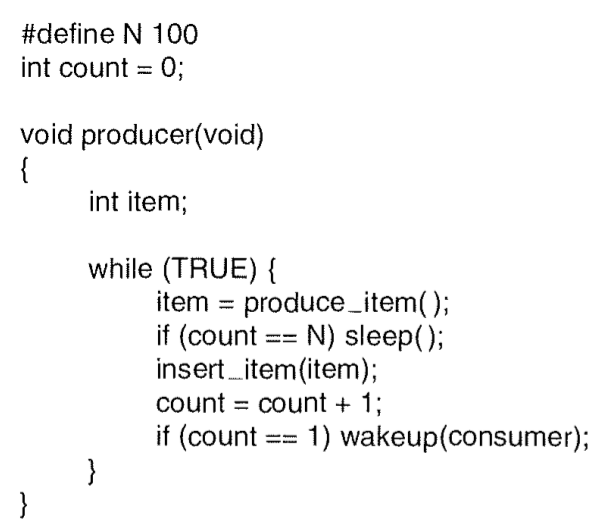
\includegraphics[width=1.0\textwidth]{prod.png}
\column{.5\textwidth}
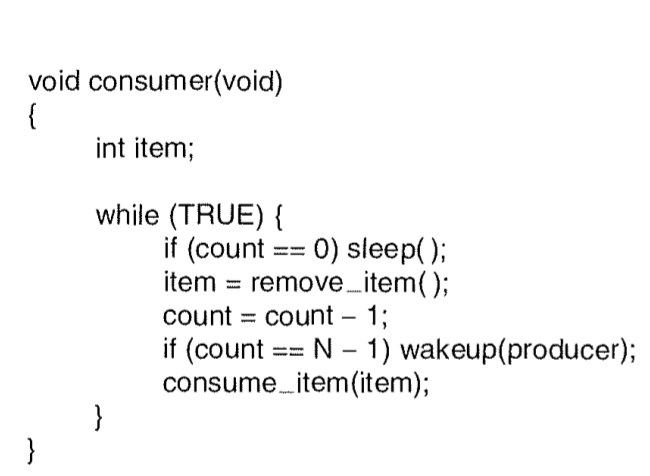
\includegraphics[width=1.0\textwidth]{consum.png}
\end{columns}%[t]

竞争条件:消费者进程测试count==0成功后、调用sleep之前,调度生产者进程运行
\end{frame}

\begin{frame}{信号量机制(Semaphores)}
为了解决唤醒信号丢失的问题,引入信号量,它是一种特殊的整型变量。在信号量上定义两个\alert{原子操作}:
\begin{description}
\item[down]  如果信号量值大于0,则将其减1然后返回;否则,进程在该信号量上进入睡眠
\item[up]  如果有进程在该信号量上睡眠,则选择其中一个唤醒;否则,信号量加1 
\end{description}
\end{frame}

\begin{frame}{用信号量解决生产者--消费者问题}
\begin{columns}[b]
\column{.5\textwidth}
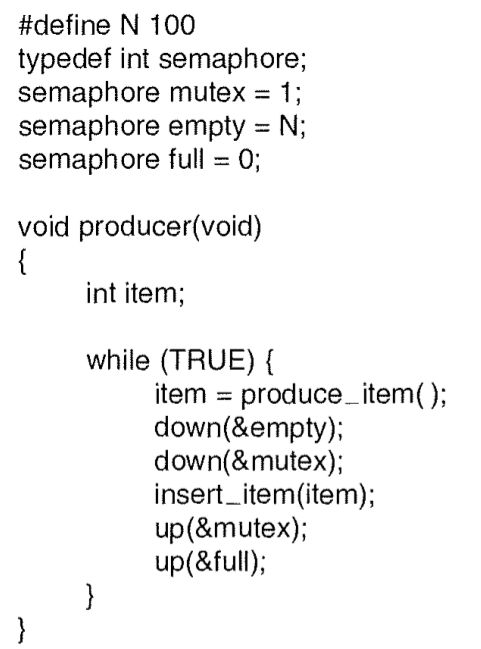
\includegraphics[width=1.0\textwidth]{prodsem.png}
\column{.5\textwidth}
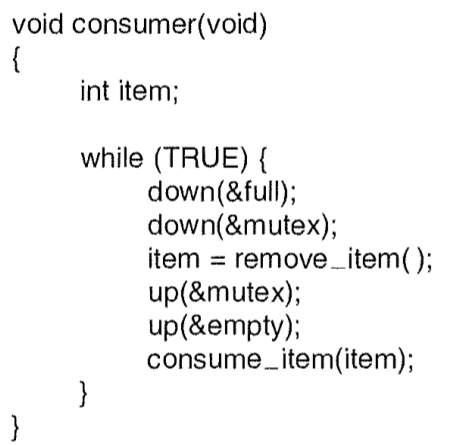
\includegraphics[width=1.0\textwidth]{conssem.png}
\end{columns}%[t]

该方案中,信号量empty和full具有计数和同步功能,而mutex仅有互斥功能。
\end{frame}

\begin{frame}{专门用来实现互斥的特殊信号量 -- 互斥锁}
互斥锁只有两种状态:locked (1) / unlocked (0)

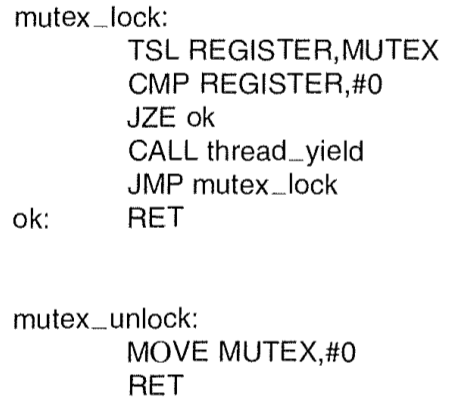
\includegraphics[width=0.5\textwidth]{mutex.png}
\end{frame}

\begin{frame}{信号量的危险情形 --- 管程机制的引入}
\begin{columns}[b]
\column{.5\textwidth}
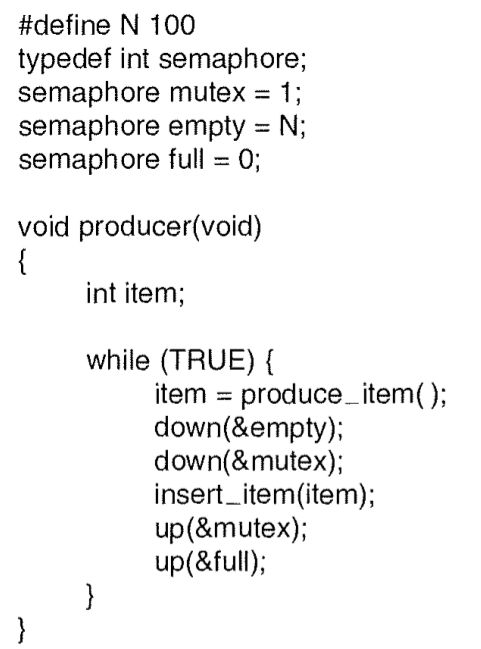
\includegraphics[width=1.0\textwidth]{prodsem.png}
\column{.5\textwidth}
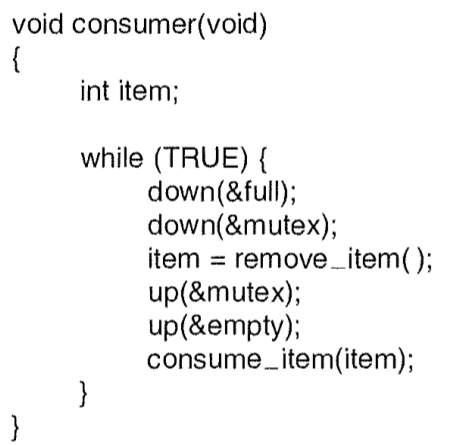
\includegraphics[width=1.0\textwidth]{conssem.png}
\end{columns}%[t]

如果把producer中的down(empty)和down(mutex)顺序颠倒,则当缓冲区满时,会发生什么?
\end{frame}

\begin{frame}{管程:解决生产者--消费者问题}
\begin{columns}[b]
\column{.5\textwidth}
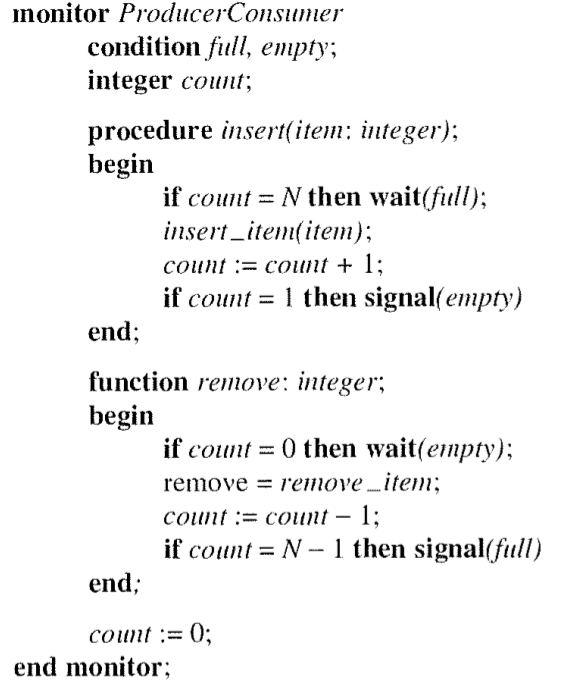
\includegraphics[width=1.0\textwidth]{mon1.png}
\column{.5\textwidth}
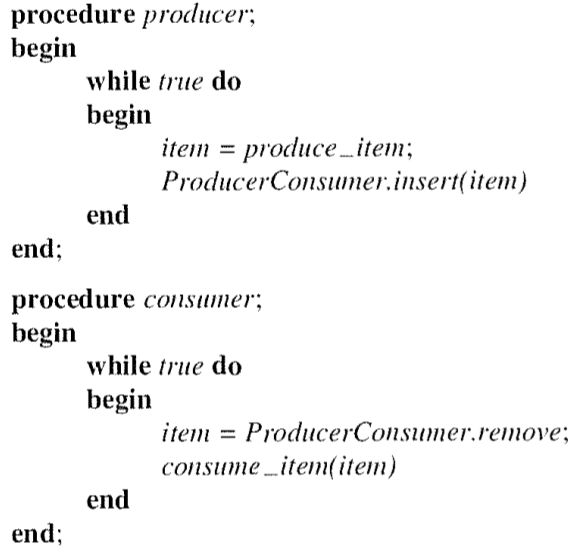
\includegraphics[width=1.0\textwidth]{mon2.png}
\end{columns}%[t]

\alert{注意概念:} 条件变量empty, full以及wait, signal

此外,insert与remove之间的互斥由编译器完成
\end{frame}

\begin{frame}{管程:解决生产者--消费者问题}
\begin{itemize}
\item 管程内程序段之间的互斥(自动)
\item 进程同步问题?:条件变量及wait, signal实现
\begin{itemize}
\item wait: 将当前进程阻塞,并允许其他进程进入管程
\item signal: 将被相应条件变量阻塞的进程唤醒
\end{itemize}
\item 上述方法中,signal必须是最后一条指令,为什么? 
\end{itemize}
\end{frame}

\begin{frame}{进程(线程)调度}
当系统中有多个进程或线程处于就绪态时,操作系统需要从中选择一个放到CPU上运行。
这就是进程调度问题。实现该任务的部件称作调度器。
\end{frame}

\begin{frame}{进程的典型行为: CPU密集型与IO密集型进程}
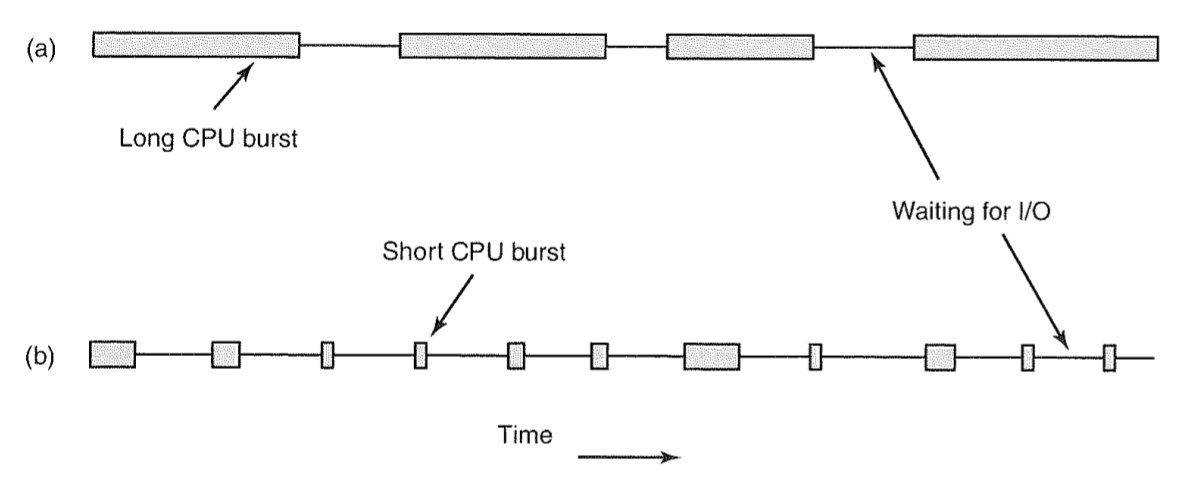
\includegraphics[width=1.0\textwidth]{behav.png}

思考:两种进程举例?

二者关键区别:不是I/O时间长度,而是CPU时间长度
\end{frame}

\begin{frame}{进程的典型行为: CPU密集型与IO密集型进程}
基本想法:如果某I/O进程处于就绪态,则应该努力优先让其运行。为什么?(这里有个深刻原因)
\end{frame}

\begin{frame}{进程调度的时机:何时调度?}
\begin{enumerate}
\item 新进程创建时,是继续运行父进程,还是运行新创建的子进程?
\item 当前进程退出时,CPU空闲,此时需从就绪态进程集合中选择一个运行
\item 当前进程阻塞时(I/O或者信号量引起)
\item 当发生I/O中断时,由此I/O信号导致阻塞的进程进入就绪态
\end{enumerate}
\end{frame}

\begin{frame}{抢占式调度与非抢占式调度}
\begin{itemize}
\item 时钟硬件中断信号的频率大约为50~60Hz
\item 在1个或者K个时钟中断信号处,强迫终止当前运行的进程。这类调度称为抢占式调度
\item 非抢占式调度:进程一旦运行,则除非它阻塞或者自愿放弃CPU,不剥夺其CPU使用权。
\item 抢占式调度用于分时系统;需要\alert{时钟硬件}的支持
\end{itemize}
\end{frame}

\begin{frame}{进程调度算法}
\begin{columns}
\column{.4\textwidth}
\begin{itemize}
\item 时间片轮转调度
\begin{itemize}
\item 公平、简单
\item 关键数据结构:队列
\end{itemize}
\item 优先级调度
\begin{itemize}
\item 基本假定是有些进程比其他进程重要
\item 关键数据结构:\alert{优先队列}
\end{itemize}
\item 优先级与时间片轮转相结合
\end{itemize}
\column{.6\textwidth}
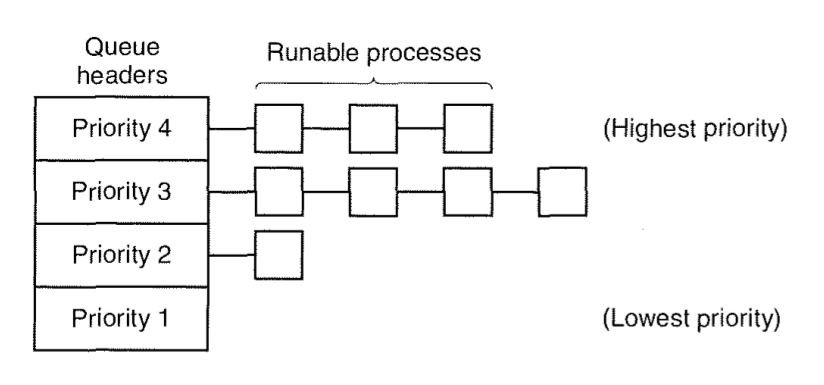
\includegraphics[width=1.0\textwidth]{comb.png}
\end{columns}
\end{frame}

\begin{frame}{内存管理器(Memory Manager)的任务}
\begin{itemize}
\item 提供内存抽象界面
\item 分配物理内存,回收物理内存
\item 记录内存使用情况等
\end{itemize}
\end{frame}

\begin{frame}{没有内存抽象:程序员直接操作物理内存}
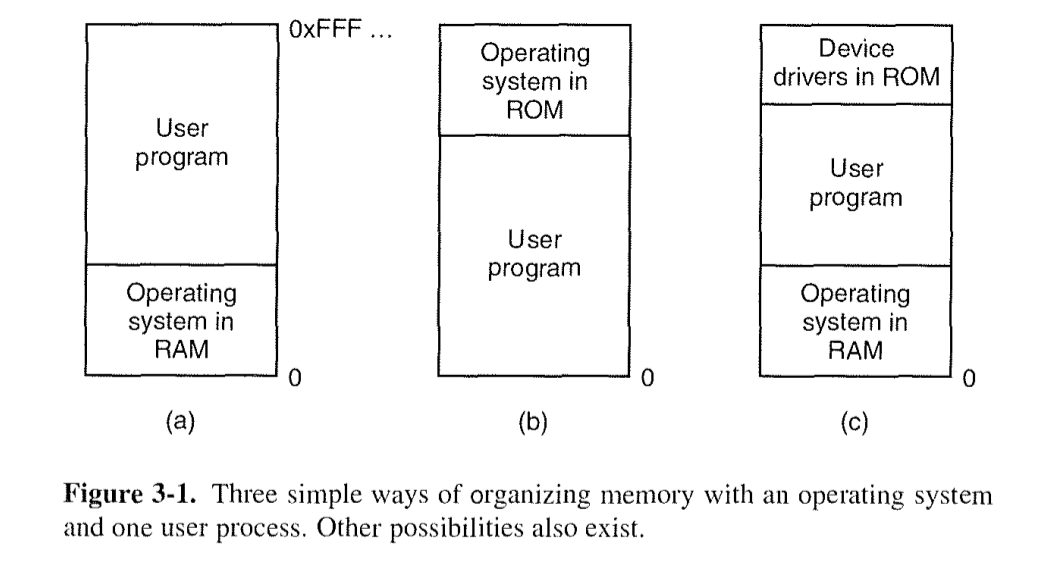
\includegraphics[width=1.0\textwidth]{nomem.png}

a. 内存中一次只能驻留一个程序:\alert{MOV REGISTER1, 1000}

b. 操作系统自身代码难以保护(没有地址空间概念)
\end{frame}

\begin{frame}{虚拟内存技术}
%虚拟内存技术可解决个问题:
\begin{itemize}
\item 问题一:如何让多个程序驻留内存?
\begin{itemize}
\item 每个程序有专属地址空间
\item 程序不能非法访问其他程序的地址空间
\end{itemize}
\item 问题二:如何满足程序对内存的无限需求?
\begin{itemize}
\item 地址空间分成若干\alert{页面}
\item 地址空间的页面映射到物理内存的\alert{页框}内
\item 利用\alert{页表}实现页面号到页框号的映射
\item 不是所有的页面都需要放到物理内存中
\item 缺页中断技术
\end{itemize}
\end{itemize}
\end{frame}

\begin{frame}{虚拟内存技术}
分页技术的精髓:不是所有页面都需要同时调入内存
\end{frame}

\begin{frame}{虚拟地址、物理地址及内存管理单元}
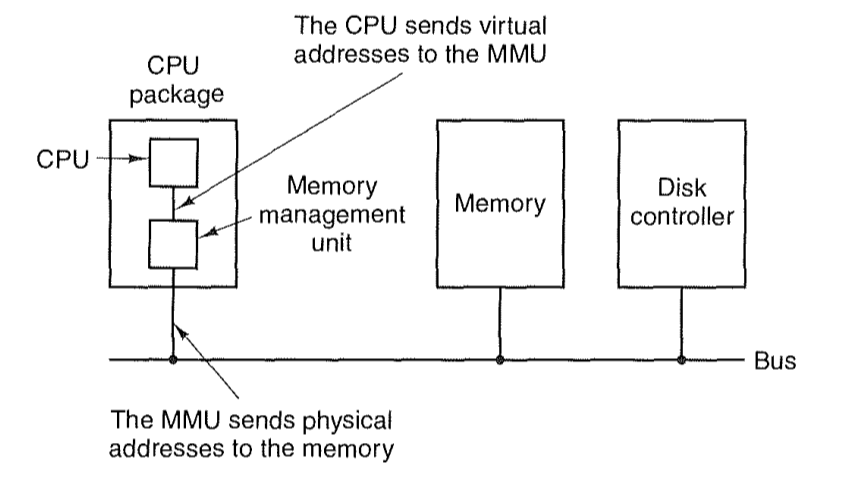
\includegraphics[width=0.9\textwidth]{mmu.png}

\alert{注意}:程序中的地址全都是虚拟地址
\end{frame}

\begin{frame}{虚拟地址、物理地址及内存管理单元}
\begin{columns}%[t]
\column{.4\textwidth}
\begin{itemize}
\item 虚拟地址空间:64K (16 bit)
\item 物理地址空间:32K (15 bit)
\item 页面大小:4K 
\item 共16个(虚拟)页面,8个(物理)页框
\item 对于大于32K的程序,只能有32K驻留物理内存(右图数字部分)
\end{itemize}
\column{.6\textwidth}
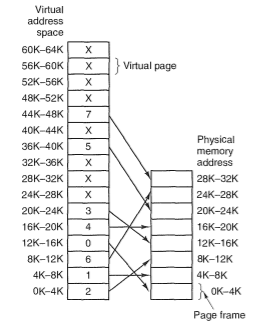
\includegraphics[width=1.0\textwidth]{vm.png}
\end{columns}%[t]
\end{frame}

\begin{frame}{虚拟地址、物理地址及内存管理单元}
\begin{columns}%[t]
\column{.4\textwidth}
\begin{block}{MOV REG, 20500}
20500 = 5 * 4K + 20 

页面5 $\rightarrow$ 页框3

12K + 20 = 12308(物理地址)
\end{block}
\begin{block}{MOV REG, 32780}
32780 = 8 * 4K + 12

对应虚拟页面8(缺页)

\alert{what next?}
\end{block}
\begin{block}{页表内容}
需要由操作系统维护
\end{block}
\column{.6\textwidth}
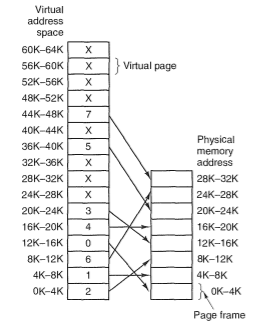
\includegraphics[width=1.0\textwidth]{vm.png}
\end{columns}%[t]
\end{frame}

\begin{frame}{虚拟地址、物理地址及内存管理单元}
\begin{columns}%[t]
\column{.4\textwidth}
虚拟地址映射到物理地址,考虑右图例子:
\begin{itemize}
\item 页面大小:4K 
\item 页内地址为12位
\item 对于16位机器而言,有4位用于页表索引
\item 因此共有16个虚拟页面
\item 8个物理页框(需3位)
\end{itemize}
\column{.6\textwidth}
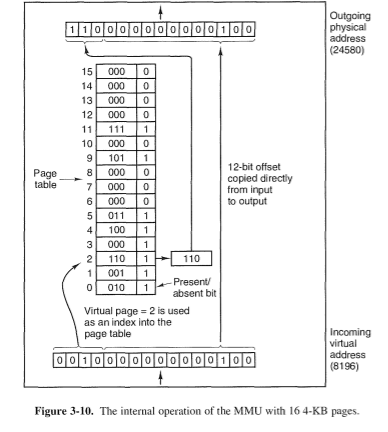
\includegraphics[width=1.0\textwidth]{mmu2.png}
\end{columns}%[t]
\end{frame}

\begin{frame}{页表项}
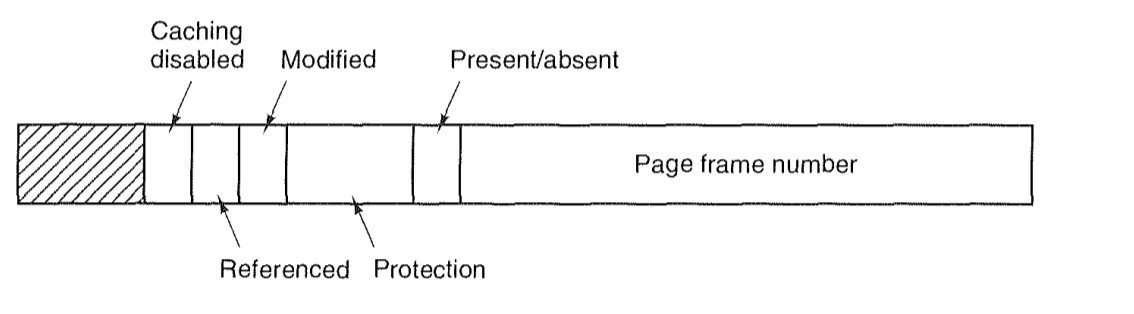
\includegraphics[width=1.0\textwidth]{pte.png}
\begin{description}
\item[page frame number]描述该页表项对应的页框编号
\item[present / absent]表示该页表是否在内存中
\item[protection]含读、写、执行等权限信息
\item[modified]该页表内容是否被修改过
\item[referenced]该页表内容是否被用过(读写)
\item[caching disabled]用于memory mapped I/O(后续)
\end{description}
\end{frame}

\begin{frame}{虚拟内存技术与分页技术面临的两大问题}
\begin{enumerate}
\item 从虚拟地址到物理地址的映射必须快
\begin{itemize}
\item 每条指令都需从内存取出
\item 大量指令涉及读写内存(CISC机器)
\end{itemize}
\item 如果虚拟地址空间很大,则页表规模会特别大

考虑页面大小4K的虚拟内存系统:
\begin{itemize}
\item 32位虚拟地址: 100万个页表项
\item 64位虚拟地址:45035996亿个页表项
\item 注意:每个进程都需要单独的页表!!
\end{itemize}
\end{enumerate}
\end{frame}

\begin{frame}{从虚拟地址到物理地址的快速映射:TLB(联想式存储)}
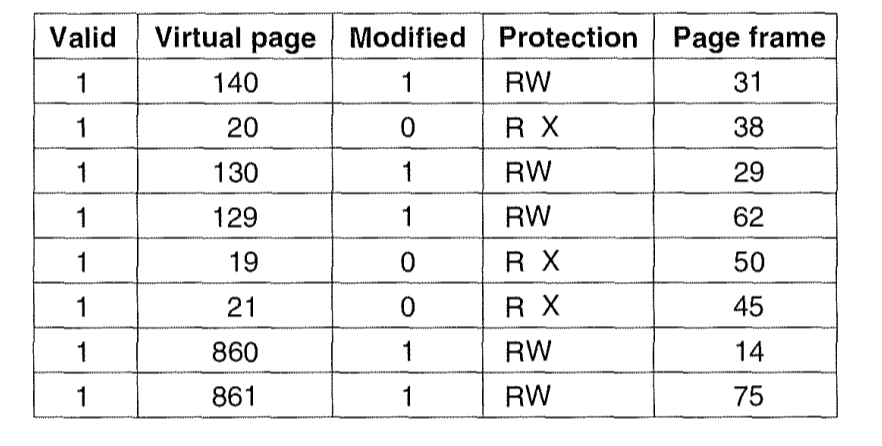
\includegraphics[width=1.0\textwidth]{tlb.png}

放置在MMU里面。来虚拟地址,先查TLB。
\begin{itemize}
\item 若能在TLB中查到该虚拟地址,则直接输出物理页框号码
\item 否则,去内存中的页表中查找对应页框号码,并将其调入TLB
\end{itemize}
\end{frame}

\begin{frame}{处理大规模地址空间的方法一:多级页表}
%\begin{columns}%[t]
%\column{.3\textwidth}
%多级页表:页表的全部内容不必都放在内存中
%\column{.7\textwidth}
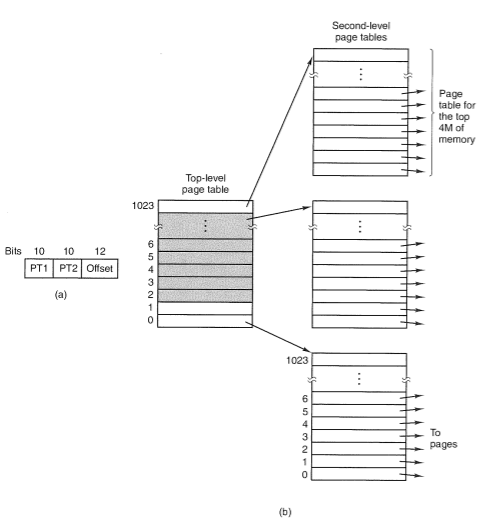
\includegraphics[width=0.7\textwidth]{multi.png}
%\end{columns}%[t]

多级页表:页表的全部内容不必都放在内存中
\end{frame}

\begin{frame}{处理大规模地址空间的方法二:倒排页表}
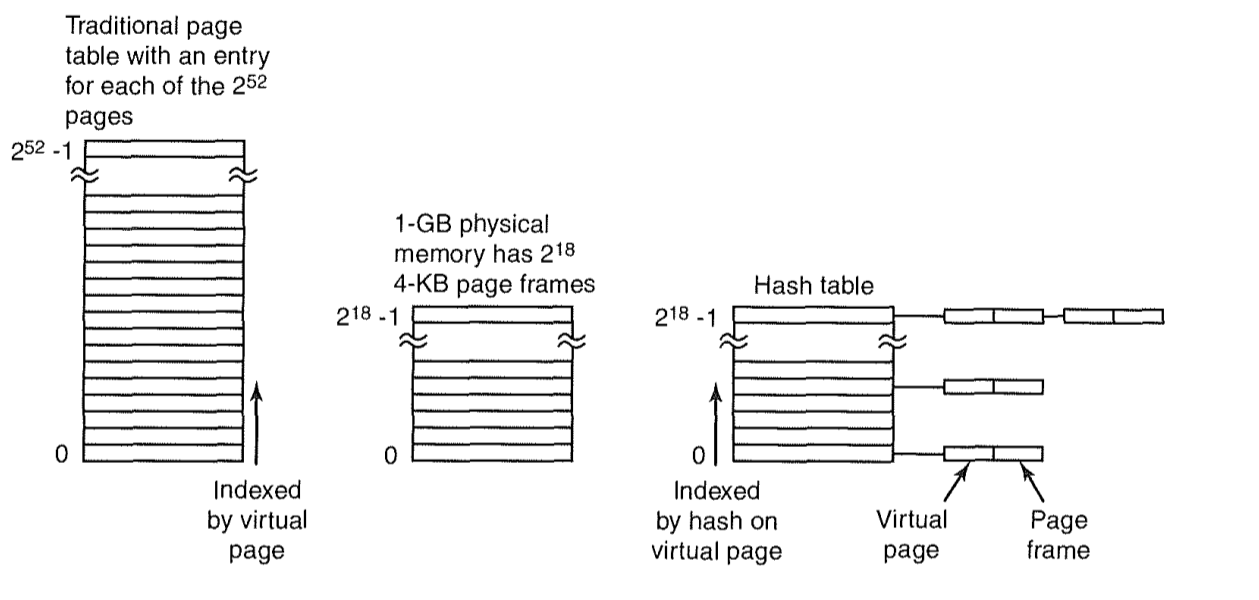
\includegraphics[width=1.0\textwidth]{inverted.png}
\end{frame}

\begin{frame}{页面置换算法}
当发生缺页时,OS需要选择一个页面将其从物理内存转移至硬盘,然后从硬盘调入所缺页面。
\end{frame}

\begin{frame}{老化(aging)页面置换算法}
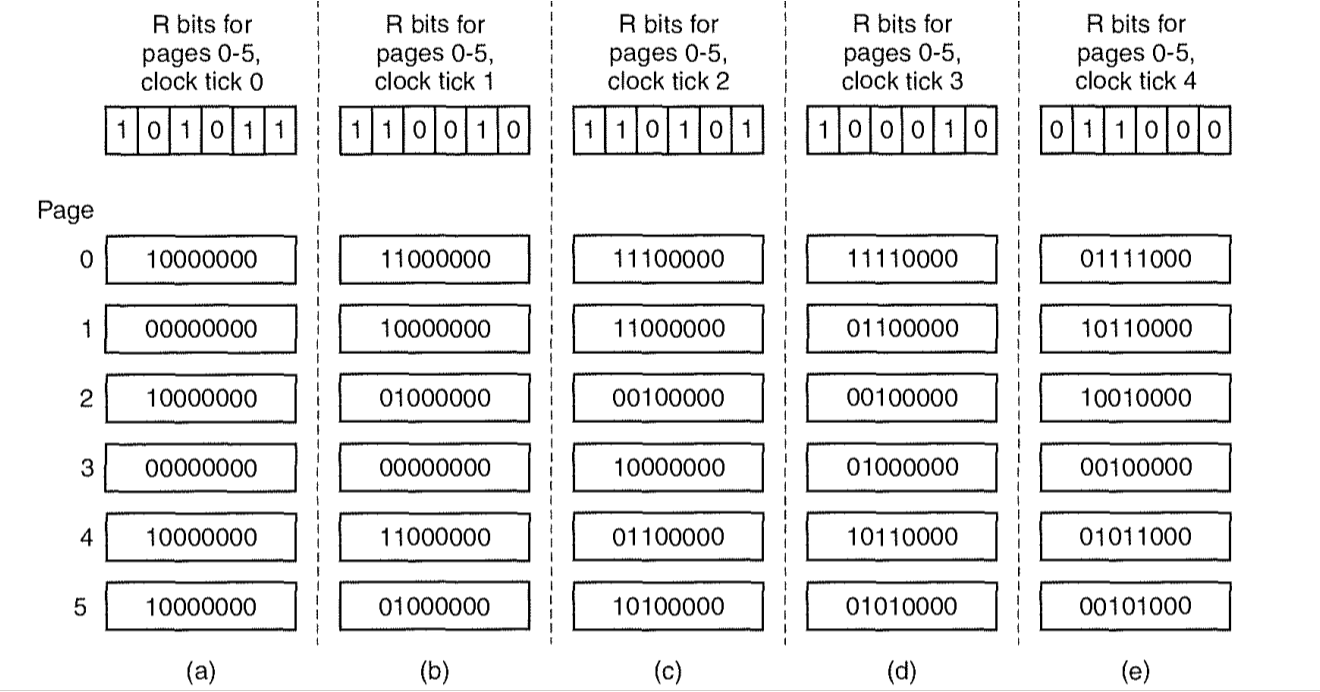
\includegraphics[width=1.0\textwidth]{aging.png}
\end{frame}

\begin{frame}{工作集(working set)页面置换算法}
\begin{itemize}
\item 访问的\alert{局部性}:在任一时间段内,程序仅仅访问其所有页面的一小部分。
\item[]
\item 我们将程序在某时间段内密集访问的页面集合成为\alert{工作集}
\end{itemize}
\end{frame}

\begin{frame}{工作集(working set)页面置换算法}
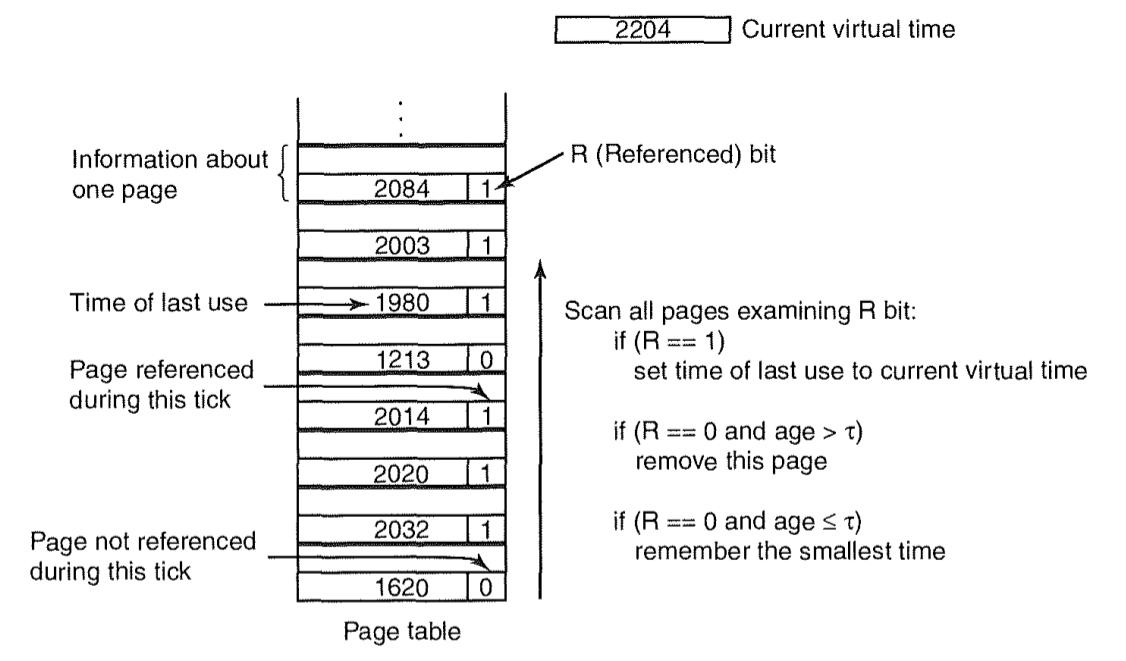
\includegraphics[width=1.0\textwidth]{ws.png}

思考:如果找不到不在工作集的页面,怎么办?
\end{frame}

\begin{frame}{单纯分页技术的缺点--分段技术的引入}
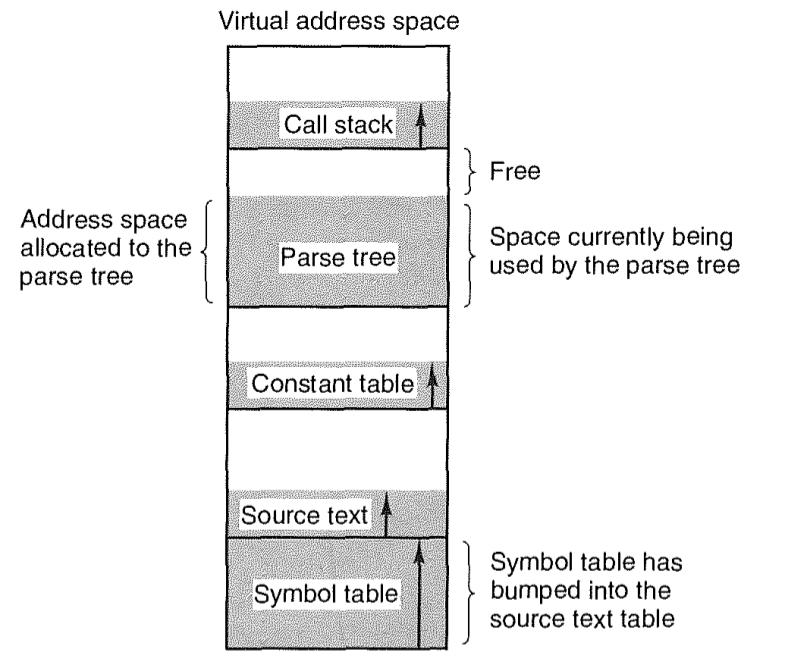
\includegraphics[width=0.7\textwidth]{noseg.png}
\end{frame}

\begin{frame}{单纯分页技术的缺点--分段技术的引入}
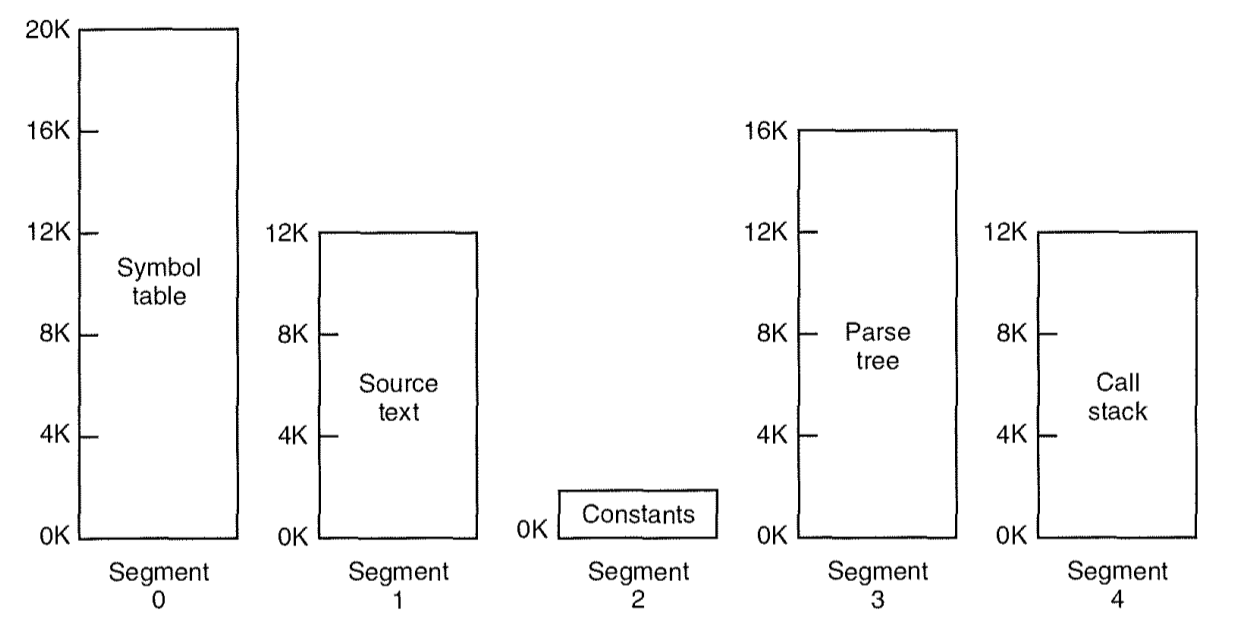
\includegraphics[width=1.0\textwidth]{seg.png}

每个段(segment)是独立的地址空间,互不干涉,可自如伸缩
\end{frame}

\begin{frame}{分段技术}
\begin{itemize}
\item 程序员(编译器)可见
\item 每个段可以对应子函数、栈、数组、其它类型变量中的一种(但一般不是多种)
\item 分段以后,更有利于保护(代码段--执行、数据段--读写)
\item 分段以后,更便于在进程间共享代码与数据
\end{itemize}
\end{frame}

\begin{frame}{分段与分页技术相结合 --- 融合二者优点}
如果某个段(segment)特别大,无法全放入内存,怎么办?

\alert{答案}:针对每个段,采用分页技术。即只把每段中部分页面放入物理内存
\end{frame}

\begin{frame}{Intel平台上的分段分页技术: GDT与LDT}
Intel平台上,所有段表分成两类:
\begin{enumerate}
\item[]
\item GDT (Global Descriptor Table) -- 系统段(OS), 仅1个
\item[]
\item LDT (Local Descriptor Table) -- 每个进程都有自己的LDT
\end{enumerate}
\end{frame}

\begin{frame}{Intel平台上的分段分页技术: 段选择符(Segment Selector)}
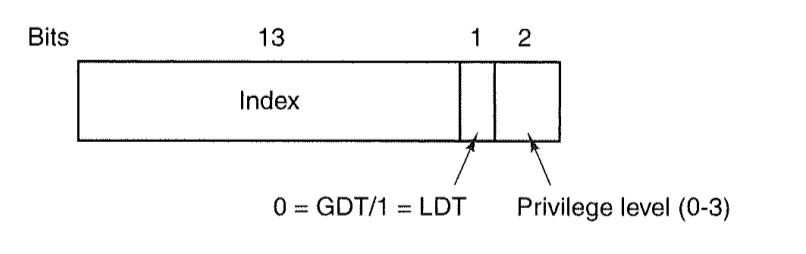
\includegraphics[width=1.0\textwidth]{selector.png}

\begin{description}
\item[CS寄存器] 存放代码段的段选择符
\item[DS寄存器] 存放数据段的段选择符
\item[其他] 四个段寄存器
\end{description}
\end{frame}

\begin{frame}{Intel平台上的分段分页技术: 段描述符(Segment Descriptor) -- 段表项}
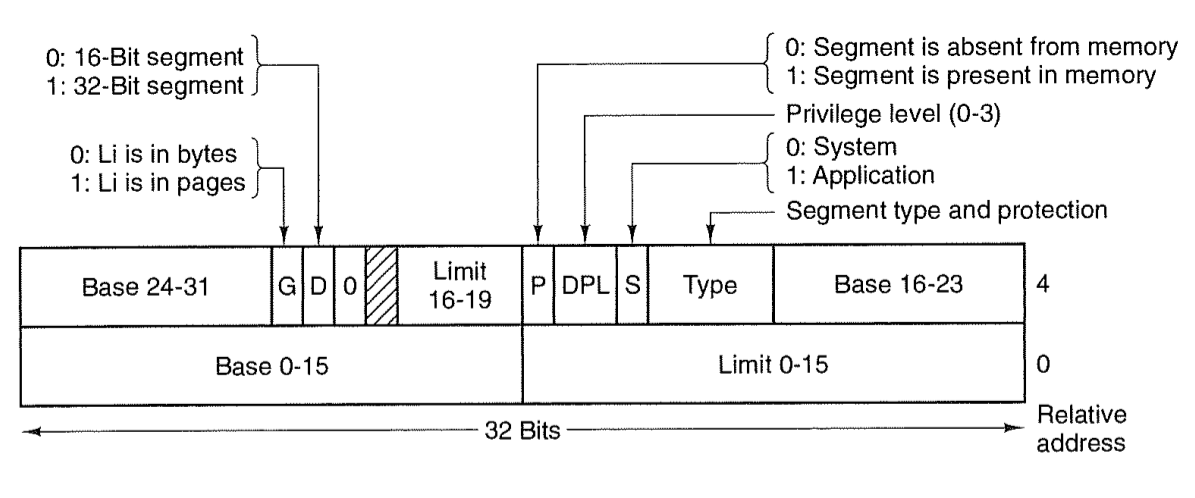
\includegraphics[width=1.0\textwidth]{descriptor.png}

三个关键字段:BASE,LIMIT,G
\end{frame}

\begin{frame}{Intel平台上的分段分页技术: 从(段选择符,偏移)到线性地址的映射}
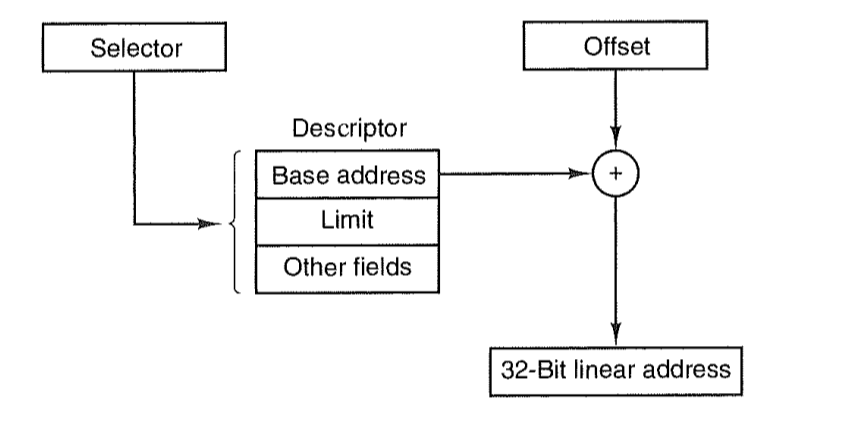
\includegraphics[width=1.0\textwidth]{smap.png}
\end{frame}

\begin{frame}{Intel平台上的分段分页技术: 从线性地址到物理地址的映射}
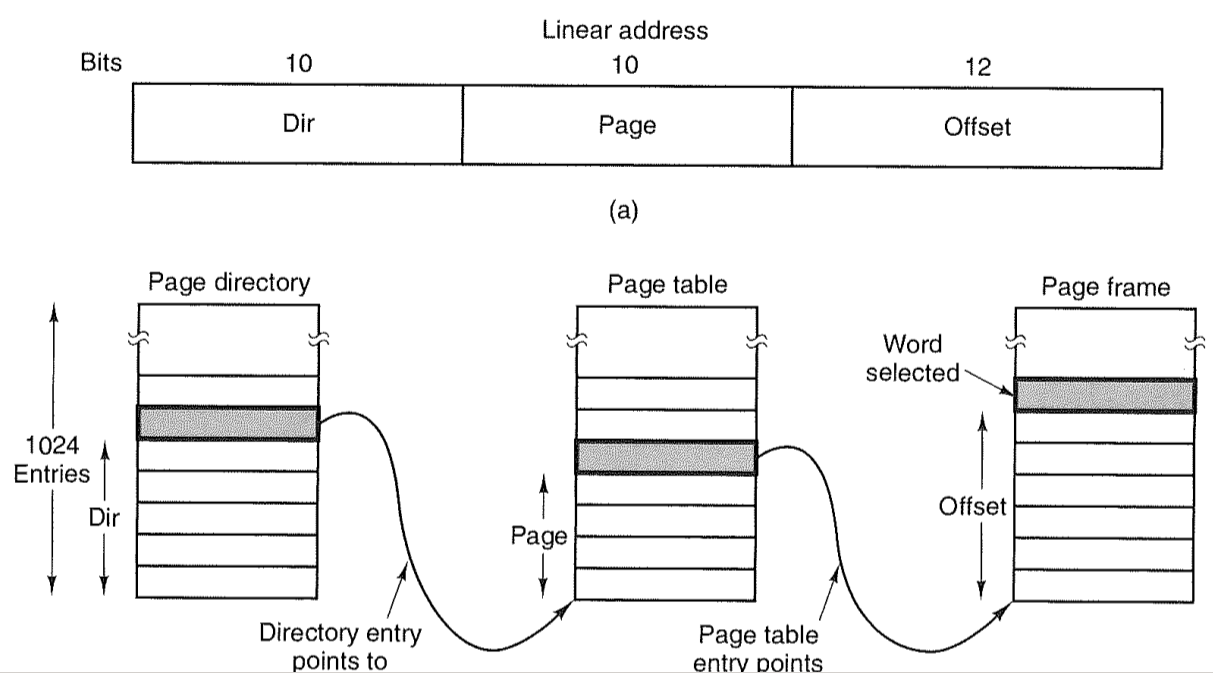
\includegraphics[width=1.0\textwidth]{pmap.png}
\end{frame}

\end{CJK*}
\end{document}
